%%%%%%%%%%%%%%%%%%%%%%%%%%%%%%%%%%%%%%%%%
% Masters/Doctoral Thesis 
% LaTeX Template
% Version 2.5 (27/8/17)
%
% This template was downloaded from:
% http://www.LaTeXTemplates.com
%
% Version 2.x major modifications by:
% Vel (vel@latextemplates.com)
%
% This template is based on a template by:
% Steve Gunn (http://users.ecs.soton.ac.uk/srg/softwaretools/document/templates/)
% Sunil Patel (http://www.sunilpatel.co.uk/thesis-template/)
%
% Template license:
% CC BY-NC-SA 3.0 (http://creativecommons.org/licenses/by-nc-sa/3.0/)
%
%%%%%%%%%%%%%%%%%%%%%%%%%%%%%%%%%%%%%%%%%

%----------------------------------------------------------------------------------------
%	PACKAGES AND OTHER DOCUMENT CONFIGURATIONS
%----------------------------------------------------------------------------------------

\documentclass[
12pt, % The default document font size, options: 10pt, 11pt, 12pt
%oneside, % Two side (alternating margins) for binding by default, uncomment to switch to one side
english, % ngerman for German
doublespacing, % Single line spacing, alternatives: onehalfspacing or doublespacing
%draft, % Uncomment to enable draft mode (no pictures, no links, overfull hboxes indicated)
nolistspacing, % If the document is onehalfspacing or doublespacing, uncomment this to set spacing in lists to single
%liststotoc, % Uncomment to add the list of figures/tables/etc to the table of contents
%toctotoc, % Uncomment to add the main table of contents to the table of contents
parskip, % Uncomment to add space between paragraphs
%nohyperref, % Uncomment to not load the hyperref package
headsepline, % Uncomment to get a line under the header
chapterinoneline, % Uncomment to place the chapter title next to the number on one line
%consistentlayout, % Uncomment to change the layout of the declaration, abstract and acknowledgements pages to match the default layout
]{MastersDoctoralThesis} % The class file specifying the document structure

\usepackage[utf8]{inputenc} % Required for inputting international characters
\usepackage[T1]{fontenc} % Output font encoding for international characters

%\usepackage{mathpazo} % Use the Palatino font by default

\usepackage[sorting=none, url=false, eprint=false,]{biblatex}
%\usepackage[backend=bibtex,,natbib=true]{biblatex} % Use the bibtex backend with the authoryear citation style (which resembles APA)

\addbibresource{example.bib} % The filename of the bibliography

\usepackage[autostyle=true]{csquotes} % Required to generate language-dependent quotes in the bibliography

\usepackage{mathtools}
\DeclarePairedDelimiter\bra{\langle}{\rvert}
\DeclarePairedDelimiter\ket{\lvert}{\rangle}
\DeclarePairedDelimiterX\braket[2]{\langle}{\rangle}{#1 \delimsize\vert #2}

\usepackage[]{titlesec} %Required to prevent hyphenation in section titles.  Options Here control chapter headings, Section Headings etc. 
\usepackage{gensymb}

%----------------------------------------------------------------------------------------
%	MARGIN SETTINGS
%----------------------------------------------------------------------------------------

\geometry{
	paper=letterpaper,  
	head=24pt,
	hmargin={1.5in,1.25in},
	vmargin=1.25in,
	twoside = true,
	}

%----------------------------------------------------------------------------------------
%	THESIS INFORMATION
%----------------------------------------------------------------------------------------

\thesistitle{Cellular Metabolism and Chemical Dynamics Through the Lens of Vibrational Microscopy} % Your thesis title, this is used in the title and abstract, print it elsewhere with \ttitle
\supervisor{Professor Eric O. \textsc{Potma}} % Your supervisor's name, this is used in the title page, print it elsewhere with \supname
\author{Richard C. \textsc{Prince}} % Your name, this is used in the title page and abstract, print it elsewhere with \authorname
\university{{University of California, Irvine}} % Your university's name and URL, this is used in the title page and abstract, print it elsewhere with \univname
\department{{Department of Biomedical Engineering}} % Your department's name and URL, this is used in the title page and abstract, print it elsewhere with \deptname

\AtBeginDocument{
\hypersetup{pdftitle=\ttitle} % Set the PDF's title to your title
\hypersetup{pdfauthor=\authorname} % Set the PDF's author to your name
%\hypersetup{pdfkeywords=\keywordnames} % Set the PDF's keywords to your keywords
}

\begin{document}

\frontmatter % Use roman page numbering style (i, ii, iii, iv...) for the pre-content pages

\pagestyle{plain} % Default to the plain heading style until the thesis style is called for the body content

%----------------------------------------------------------------------------------------
%	TITLE PAGE
%----------------------------------------------------------------------------------------

\begin{titlepage}
\begin{center}


{\scshape\large \univname\par}\vspace{.2cm} % University name
\deptname\\[.5cm] % Research group name and department name
\textsc{\large Qualifying Exam}\\[0.2cm] % Thesis type

\HRule \\ % Horizontal line
{\Large \bfseries \ttitle\par}\vspace{0.2cm} % Thesis title
\HRule \\ % Horizontal line
\vspace*{.1\textheight}
 
\begin{minipage}[t]{0.4\textwidth}
\begin{flushleft} \large
\emph{Author:}\\
{\authorname} % Author name - remove the \href bracket to remove the link
\end{flushleft}
\end{minipage}
\begin{minipage}[t]{0.4\textwidth}
\begin{flushright} \large
\emph{Supervisor:} \\
{\supname} % Supervisor name - remove the \href bracket to remove the link  
\end{flushright}
\end{minipage}\\[4cm]
 
\vfill

{\large November 13, 2018}\\[4cm] % Date
%\includegraphics{Logo} % University/department logo - uncomment to place it
 
\vfill
\end{center}
\end{titlepage}

%----------------------------------------------------------------------------------------
%	Redefine \cleardouble page to print notice of blank page.
%----------------------------------------------------------------------------------------
\newcommand*{\blankpage}{%
\vspace*{\fill}
{\centering This page is left blank with the exception of telling you that the page is intentionally left blank.\par}
\vspace{\fill}}
\makeatletter
\renewcommand*{\cleardoublepage}{\clearpage\if@twoside \ifodd\c@page\else
\blankpage
\thispagestyle{empty}
\newpage
\if@twocolumn\hbox{}\newpage\fi\fi\fi}
\makeatother


%----------------------------------------------------------------------------------------
%	THESIS CONTENT - CHAPTERS
%----------------------------------------------------------------------------------------

\mainmatter % Begin numeric (1,2,3...) page numbering

\pagestyle{thesis} % Return the page headers back to the "thesis" style

% Include the chapters of the thesis as separate files from the Chapters folder
% Uncomment the lines as you write the chapters

% Chapter 1

\chapter{Introduction \& Specific Aims} % Main chapter title

\label{Chapter1} % For referencing the chapter elsewhere, use \ref{Chapter1} 

%----------------------------------------------------------------------------------------

% Define some commands to keep the formatting separated from the content 
\newcommand{\keyword}[1]{\textbf{#1}}
\newcommand{\tabhead}[1]{\textbf{#1}}
\newcommand{\code}[1]{\texttt{#1}}
\newcommand{\file}[1]{\texttt{\bfseries#1}}
\newcommand{\option}[1]{\texttt{\itshape#1}}

%----------------------------------------------------------------------------------------
\section{Probing Biology with Vibrational Contrast}
Coherent Raman Scattering (CRS) makes up a powerful suite of tools accessible to the biomedical microscopist.  As a field, this set of imaging techniques is less than twenty years old.  However, the large number of publications from around the world as well as the inclusion of turn-key systems into commercial microscopes serve as proof of their usefulness. Under the microscope, both coherent anti-Stokes Raman Scattering (CARS) and Stimulated Raman Scattering (SRS) have been successfully utilized to image the distribution of lipids in single cells and tissues, to study the diffusion dynamics of intracellular water, to follow myelination of neurons, and to address a host of other challenges in biology and biomedicine.~\cite{Prince:2017aa, Camp-Jr:2015aa, doi:10.1002/9783527808465.EMC2016.8365}  

The majority of published findings have studied static biological features, or have observed changes over long time scales, or have imaged samples at extended time points i.e. excision of tissue from specimens of differing ages.\cite{Camp-Jr:2015aa,doi:10.1002/9783527808465.EMC2016.8365,C5CS00693G} Recent improvements in detection technology and advances in the use of isotopic and inert chemical tags have set the stage for the thorough application of vibrational imaging to the investigation of chemical dynamics in single cell systems. It is the aim of this proposal to set forth a plan of research that expands SRS toward shorter timescales, demonstrates its utility to metabolic processing and examination, and extends the palette of vibrational imaging techniques.

%----------------------------------------------------------------------------------------
\section{Specific Aims}
\subsection{Aim 1: Elucidate diffusion dynamics of common cryoprotectants}
Small molecules such as dimethyl sulfoxide (DMSO) and glycerol have been used as cryoprotectants for several decades.~\cite{Pegg:2002aa}  Their discovery as such is thought to have been accidental, but in the time since much work has been done to establish a coherent physical theory as to their ability to protect biological specimens during cryogenic storage.~\cite{Pegg2007}  It is apparent that suppression of ice crystals formation in cells is extremely important to prevent cellular damage, as is proper extracellular spacing.  However, the specific chemical dynamics of this process prior to and during freezing are not well understood.  This study seeks to address this by using isotopically labeled cryoprotectants as a probe in SRS imaging studies.  Through this work, I intend to elucidate the diffusion and permeability of the cryoprotectant through membranes, establish an understanding of sub-cellular concentration dynamics, and shed light on the selective forces that cell lines undergo during the preservation process.

\subsection{Aim 2: Demonstrate a method for metabolic sorting based on SRS imaging }
Previous work from imaging groups at Columbia, UCI, and others has demonstrated the potential for deuterium labeled metabolites such as glucose to serve as markers for metabolism generally and as specific tracers of metabolic pathways.~\cite{Hou2503, Shi:2018aa, Shi:2018ab} These methods promise to elucidate many of the metabolic dynamics present in cell systems and have the potential for tracking intercellular signaling.  In this project, I intend look past the basic science potential of this technology in order to develop a method for cell sorting and classification based on metabolic markers derived through SRS imaging.  Preliminary work on this system shows that it is possible to differentiate cell types based on the SRS intensity of characteristic vibrational bands. The primary aim of this project will be to characterize signal ratios of high intensity SRS active modes to develop a set of criteria for rapid throughput sorting.  It is anticipated that this will be accomplished by culturing cells in media supplemented with heavy water.  Those cells with increased metabolic activity are hypothesized to show increased intensity of the CD band.  This project will examine what parameters of the deuterated cell's Raman spectrum constitute the minimum requirement for accomplishing the sorting task.  The secondary objective of this collaborative effort is to develop a flow system capable of using the SRS markers for quickly identifying cells in a heterogeneous mixture.

\subsection{Aim 3: Characterize Third-Order Sum-Frequency Generation as applied to biological systems }
Previously this year, our group demonstrated a new multimodal microscope capable of rapid imaging through sum-frequency generation (SFG) and CARS.~\cite{8378261, Hanninen:18}  This system is the first to implement such an imaging scheme, and it does so through the use of near and mid-infrared (MIR) excitation beams.  The use of high-intensity narrow-band pulses in the MIR opens up a new modality in the form of third-order sum-frequency generation (TSFG).  This is a novel technique that has not been previously reported in the imaging literature.  In a series of studies, I intend to optimize this system for high throughput imaging of biological systems. This will involve the optimization of optical components and layout, as well as automation of excitation tuning.  This project also includes the validation of the TSFG method for studying biological specimens. This work is expected have an impact in the field of optical imaging, as it has the ability to probe IR-active modes as well as Raman active modes. This implies that this platform has the potential to reveal additional and complementary data relative to what is available on the CRS microscope.  

While we have shown the ability for cellular imaging with this system, the response of different chemical groups has yet to be characterized. Preliminary results show divergence in the spectra acquired on this platform as compared to the characteristic peaks found in Raman and IR-Absorbance spectra. Characterization of standard samples of cholesterol, long chain fatty acids, collagen, and others will be accomplished through polarization resolved and spectrally sensitive measurements.  In this way, our toolkit of vibrational contrast imaging will be expanded, while providing the ability to use multiple techniques on one platform.
%----------------------------------------------------------------------------------------
\section{Scope of Work}
In this proposal, the research opportunities presented by nonlinear vibrational microscopy are outlined and explored.  Previous work has focused extensively on the distribution of lipids and other vital compounds throughout cells, the distribution of drugs through tissue layers, and the properties and motion of intracellular water.  Here, I propose a series of experiments to extend the functional toolkit available through use of SRS.  First, SRS is used to explore a fundamental science question.  The physical aspects of small molecule cryoprotectants is not well understood.  Through the use of DMSO and glycerol effusion experiments under the microscope, the dynamics at play in during the diffusion process will be elucidated. Second, a question of applied science is addressed by providing a translatable use of SRS.  The ability of SRS to quickly sample individual peaks in the Raman spectrum provides an opportunity to metabolically analyze heterogeneous cell cultures and provide chemical labeling to the cells within.  This method will then be applied to perform cell sorting in a microfluidic sorting system.  Finally, a new modality in the family of vibrational imaging techniques is developed and explored.  Characterization of the TSFG signal produced in organic compounds and biological specimens will require optimization of a new microscope system.  The virtue of this work will become evident as new information obtained from the IR-active modes of molecules will extend our imaging ability.

The work outlined above provides a pathway to the completion of my doctoral dissertation.  The first chapter of that work has already been obtained through the publication of a review article outlining the state of the field of SRS.~\cite{Prince:2017aa} A second chapter detailing my work on isotopic probes in newly a newly characterized cell type, the lipochondrocyes, and the applicability of these probes to studying metabolic pathways is currently summarize in a manuscript that is expected to be submitted before the end of the year.  Each project detailed above will constitute an additional chapter of the dissertation, and in this way will represent a body of original work that extends the field of vibrational imaging and provides new scientific information on the physics at play in several biological systems.


% Chapter Template

\chapter{A Brief Introduction to  Coherent Raman Scattering} % Main chapter title

\label{Chapter2} % Change X to a consecutive number; for referencing this chapter elsewhere, use \ref{ChapterX}


%----------------------------------------------------------------------------------------
%	SECTION 1
%----------------------------------------------------------------------------------------
\section{A Brief History of Nonlinear Microscopy}
Since the invention of the microscope, the role of optics in understanding biology and medicine has been difficult to overstate. During the middle and late twentieth century, many new techniques such as phase-contrast, differential interference contrast, and darkfield contrast were developed that expanded the role of microscopy and opened many new aspects of the microscopic world to investigation. The first theoretical prediction of multiphoton phenomena occurred in 1931, and the first demonstration was not until after the invention of the laser enabled access to high energy density, coherent sources of light.~\cite{Mayer31,PhysRevLett.7.229} Afterwards, nonlinear microscopy techniques, e.g. second harmonic generation (SHG), two-photon excited fluorescence (TPEF), third-harmonic generation (THG), were   developed at the turn of the twenty-first century, evolving from experimental work done in spectroscopy and laser development over the preceding decades. \cite{HELLWARTH1974318,Fine:71,Freund:86,Denk73}

During this same period, the development of Raman spectroscopy and its use as a microscopic tool accompanied the invention of the  various refractive contrast methods, harmonic generation spectroscopies, and many fluorescence techniques.~\cite{RAMAN:1928aa, doi:10.1002/jrs.1486}  Raman spectroscopy provides a means of studying the chemical constituents of a sample. The information available in a Raman experiment includes chemical subgroups, their relative concentration to one another, bond strength and dynamics, and molecular symmetry.  Raman spectroscopy is often said to give a \textit{fingerprint} from which to identify molecules.~\cite{doi:10.1080/05704928.2014.923902}  Raman has proven to be a powerful tool in many areas including gas phase, condensed matter, and more recently biology.  However, it it not without its weaknesses.  Raman measurements are notoriously slow, and it is often difficult to extract the weak Raman scattering signal from a large fluorescent background.  

The origin of the Raman effect is inherently found within quantum mechanics, and it is within that framework that several alternatives to it can be found. Much as G{\"o}ppert-Mayer predicted multiphoton absorption and emission to act as counterpart to linear absorption and fluorescence, so to were a set of phenomena analogous to Raman scattering discovered and characterized.~\cite{PhysRevLett.9.455, PhysRevLett.11.160, PhysRev.130.1850} Of particular note, are Coherent Anti-Stokes Raman Scattering (CARS) and Stimulated Raman Scattering (SRS). Collectively, they fall into the classification of Coherent Raman Scattering (CRS) techniques.  These two phenomenon provide information that is based on to the linear Raman spectra, but rely on different experimental parameters.  Depending on the information to be obtained, these experiments can often lead to quicker examination of a sample. 

Much as application of harmonic generation and two-photon fluorescence into the biologist's microscope lagged behind their spectroscopic applications, the first application of CRS technology towards a biological problem did not occur until 1999.~\cite{PhysRevLett.82.4142} Following this successful demonstration of a CARS microscope, the field of CRS imaging bloomed with many studies being published over the next decade.~\cite{Potma:2001aa, Cheng:2004aa, Evans:2008aa} SRS as a phenomenon had been demonstrated almost as soon as the laser had been invented. It was quickly realized that it could be harnessed as a technique to shift the frequency of a laser line. This field of work has seen significant progress, and it has been applied in the field of optics communication and in Raman-based fiber lasers.  

However, its application as a spectroscopic and/or microscopic tool significantly lagged. The first demonstration of an SRS microscope occurred in 2007, and was quickly followed the next year with an application to biological systems.~\cite{Ploetz2007, Freudiger1857}  Since these first demonstrations, the applicability of SRS microscopy to address fundamental and applied biological questions has been clearly demonstrated with many contributions from several different research groups and a number of review articles.~\cite{Prince:2017aa, C5CS00693G, FU201724}  Recently several groups, including ours, have pioneered the application of isotopic and small functional group tags in SRS.~\cite{C8AN00910D, Hou2503,Wei:2016aa, Alfonso-Garcia2015}

\section{Overview of the Theory of Coherent Raman Scattering}

An extended version of this section can be found in:

R. C. Prince, R. R. Frontiera, and E. O. Potma, "Stimulated Raman Scattering: From Bulk to Nano", \textit{Chemical Reviews} {\bf117}(7), 2017, 5070--5094

SRS is one of a group of third-order nonlinear interactions that arise from the interaction of high intensity light fields with matter.  By taking the perspective of the light fields, it is easy to see the connection to linear Raman scattering.  From there, it is possible to examine the interaction from a semi-classical point of view; wherein the light is viewed in the classical field picture, but the material properties are described quantum mechanically.

\begin{figure}[h]
    \centering
    \includegraphics[width=.9\textwidth]{Figures/jablonski}
    
    \caption{Schematic of the SRS light–matter interaction. (a) Jablonski diagram in the intensity representation showing the absorption of an $\omega_1$ photon and the emission of a $\omega_2$ photon. In all cases, the states $\ket{n}$ and $\ket{n'}$ are dummy states that can be representative of the mediating virtual state. (b) Field Representation diagram Fields $E_1$ and $E_2$ interact with the quantum mechanical states of the material. Note that the arrows are not time-ordered. (c) Double sided Feynman diagram of one of the SRS pathways. \label{fig1}}
    
\end{figure}

In the linear Raman process, light incident on a material scatters inelastically. The light can either excite vibrational motion in the material in which energy is loss from the field causing the light to shift to longer wavelengths, a process known as Stokes scattering, or the light can absorb energy from existing vibrations in the material, a process known as anti-Stokes scattering.  In the situation of Stokes scattering, is is fairly easy to understand that for a given incident light field with frequency $\omega_1$ the generation of vibrational motion in the sample at a resonant frequency $\omega_R$ will result in the annihilation of and $\omega_1$ photon and generation of a red-shifted photon at frequency $\omega_2$. The difference in energy of the incident and scattered photon $\hbar(\omega_1-\omega_2)$ is equal to the energy of the vibrational mode $\hbar\omega_R$.  This is shown diagrammatically in \ref{fig1} in which the incident photon at $\omega_1$ is absorbed and a Stokes photon at $\omega_2$ is emitted.  This process happens simultaneously and is said to be mediated through the virtual state, $\ket{n}$.  The mediation of the virtual state is what allows this process to occur even though there is often no electronic eigenstate that coincides with the energy of the incident light.

Raman in an inherently weak process. Of the light incident on a given sample nearly all of it is scattered elastically through Rayleigh scattering.  In Raman, the scattered photon must be provided by the vacuum field.  In terms of the occupation number of the photon modes, the Raman process changes the occupation number of the $\omega_1$ mode originally $n_1>>1$ to $n_1-1$, and the occupation of the $\omega_2$ mode, originally $n_2=0$, to $n_2+1$.  The Jablonski diagram for stimulated Raman scattering is the same as for linear Raman, and is shown in its intensity form in \ref{fig1} panel a.  However, in SRS the $\omega_2$ field is populated by a large number of photons, $n_2>>1$.  In SRS, the rate of photon generation in the $\omega_2$ channel, $W_{stim}$, is proportional to both the $n_1$ and $n_2$ occupation numbers, i.e. $n_1(n_2+1)$~\cite{Hellwarth1963}. On the other hand, for spontaneous Raman scattering the rate of emission, $W_{spon}$, is proportional to $n_1$, because $n_2=0$. The effect of the stimulating field is thus to increase the rate of $\omega_2$ emission~\cite{Crampton2016}:
\begin{equation}
\frac{W_{stim}}{W_{spon}}\propto n_2 + 1\label{eq:stimspon}
\end{equation}
As shown above, the high population number of the $\omega_2$ field greatly increases the rate of conversion of photons from the $\omega_1$ beam to the $\omega_2$.  In fact, the stimulation effect allows for information about the Raman transition to be retrieved at at a rate many orders of magnitude faster than in linear Raman scattering. This process has been dubbed stimulated Raman scattering as it is analogous to the stimulated fluorescence emission most notably responsible for the coherent production of lights in lasers. It has been demonstrated that the typical increase in signal acquisition rate from a microscopic probing volume typically exceeds $10^5$ for SRS over spontaneous Raman. In this limit, SRS offers clear benefits. For instance, if a spontaneous Raman measurement of a particular vibrational mode takes 100 ms, SRS can provide the same information with comparable S/N in only 1 $\mu$s.  

With the annihilation of an $\omega_1$ photon and emission of an $\omega_2$ photon there is a simultaneous excitation of a vibrational mode in the material. While the intensity diagram is useful for understanding the process, it does not give an entirely clear picture.  Panel b in \ref{fig1} underscores the nonlinear nature of the SRS process by showing the scattering event in terms of the electric fields involved (as opposed to the photon energies).  From this it is clear that SRS is a four-wave mixing process. By keeping track of these fields and their interactions in a time-ordered fashion, it is possible to understand the evolution of quantum coherence within the material.  

While a full quantum dynamical treatment is beyond the scope of this work, it is useful to describe the process represented by panel c in \ref{fig1}. The system starts out in the ground state, indicated by the $\left|a\right>\left<a\right|$ population at the bottom of the diagram. The first light-matter interaction is with the field of frequency $\omega_1$, which changes the bra from $\left<a\right|$ to $\left<n'\right|$. The states indicated by $n$ and $n'$ can be either real or virtual states. For ground state SRS, these electronic states are virtual states and the $n,n'$ labels are dummy indices. The second field interaction on the bra side generates the coherence $\left|a\right>\left<b\right|$. This is the Raman coherence in the material which, in the absence of fields, evolves according to the unperturbed Hamiltonian $\hat{H}_0$. The density matrix $\rho_{ab}$ is said to propagate during this period, tracking the time-dependent material response to the light-induced superposition of the ground state and the vibrationally excited states. The density matrix is then interacting with fields $\omega_1$ and $\omega_2$ on the ket side, generating the population $\left|b\right>\left<b\right|$.

When the $\omega_1$ and $\omega_2$ fields are coincident in time, the SRS process is instantaneous on the timescale of the vibrational coherence. This implies that the emitted field maintains a definite phase relation with the incident light fields. As a consequence, the SRS signal is coherent. Since this is true for every scatterer in the excitation volume, the combined radiation from the scatterers exhibits coherence as well. Spatial coherence within the excitation volume results in the coherent propagation of the signal in the so-called phase matched direction, i.e. the direction in which the radiating scatterers produce fields that are in-phase. To summarize from this diagram, the SRS interaction has moved population from the ground state to the first vibrationally excited state, and in doing so produced a coherent signal that will propagates into the far-field along the phase-matched direction. 

In order to understand the nature of the vibrationally excited states probed by both spontaneous Raman and SRS, it is necessary to examine the coupling between atoms in molecular bonds. The frequency of the incident radiation is typically in the visible to near-infrared range ($\Tilde{10^3}$ THz), whereas the frequencies of the nuclear vibrational motions in molecules are of much lower frequencies (1–100 THz). Therefore, the nuclei cannot follow the incident fields adiabatically. Instead, the molecules couple to the fields through their electrons, which can follow the rapid oscillations of the driving fields. In case there is coupling between the electron motions and the nuclear modes, the resultant electron oscillation contains information about the nuclear vibrations as well. Raman processes thus probe nuclear motions in the molecule indirectly through the motion of electrons. In SRS, the process reports on these motions through the transfer of photon energy from the $\omega_1$, or pump, beam to the $\omega_2$, or Stokes, beam. This transfer of photon energy creates two different opportunity to measure the response of the material optically in the far-field.  

\begin{eqnarray}
S_{SRG}(\omega_2)&\propto&\left|A_1\right|^2\left|A_2\right|^2Im\left\{\chi_{NL}(\Omega)\right\}\label{eq:srg}\\
S_{SRL}(\omega_1)&\propto&-\left|A_1\right|^2\left|A_2\right|^2 Im\left\{\chi_{NL}(\Omega)\right\}\label{eq:srl}
\end{eqnarray}  

Equations \ref{eq:srg} and \ref{eq:srl} show that the signal at the detector can be measured as either a gain in the Stokes beam or loss in the pump.  In both cases, the signal is linearly proportional to the intensity of the two beams as intensity is directly proportional to the square of the amplitudes of each field.  Additionally, these equations include the nonlinear response of the material through inclusion of the $\chi_{NL} (\Omega)$ term.  This is the the nonlinear susceptibility of the material and includes the fundamental selection rule for the Raman phenomenon that relates the coupling of the electron motions to the nuclear modes of the molecule.   This is shown explicitly in \ref{eq:chi} by the derivative term.  A full mathematical treatment can be found in \textit{Coherent Raman Scattering Microscopy, 2013, CRC Press}.\cite{Potma:2013aa}


\begin{equation}
\chi_{NL}(\Omega)=\frac{N}{6m\epsilon_0}\left(\frac{\partial\alpha}{\partial Q}\right)^2_0 \frac{1}{\omega^2_\nu-\Omega^2-2i\Omega\gamma}\label{eq:chi}
\end{equation}


From the theory, it is evident that SRS is capable of probing the same vibrational modes as spontaneous Raman, and in fact can do so at much higher rates.  The theory also shows that the optical effect induced in this way is capable of carrying information into the far field. At the far field, it is possible to measure the transfer of energy from one field to the other, and from this spectroscopic information can be obtained.  Knowing the spectroscopy then leads to an ability to produce contrast in an optical microscope.  

\section{The Narrowband SRS Microscope}
\begin{figure}[h]
    \centering
    \includegraphics[width=.9\textwidth]{Figures/Slide1.png}
    \caption{A Schematic Representation of the Narrowband SRS Microscope \label{scope}}
\end{figure}
The implementation of a high-resolution SRS microscope in our case is similar to other laser-scanning multi-photon systems.  A basic schematic is shown in \ref{scope}.  While it is possible to generate the SRS signal with several different excitation schemes, each has its own advantages or disadvantages.  Previous work has shown, that high spectral resolution is achieved with the use of picosecond pulses as both the Stokes and pump beams.  This allows for resolution on the order of $\sim10cm^{-1}$.  . Additionally by tuning to match specific Raman resonances such that $\Omega_R$ = $\hbar\omega_{pump}-\omega_{stokes}$ it is possible to build high resolution spectra of entire images. This capability for fast acquisition of a large spectral dataset at every pixel in an image allows for direct comparison to spontaneous Raman spectra, and the usefulness of this technique will be discussed later in this work. It is apparent from the description of the SRS process that the use of colinear picosecond pulses necessitates the use of a modulation scheme in order to resolve the rather minuscule SRL or SRG signal that propagates with the incident beams in the forward direction.

To discriminate the SRS signal from the laser light, the use of high-frequency modulation ($\sim10\;MHz)$ is required.  Modulation in this frequency range allows the SRS system to approach the shot noise limit as most laser noise occurs at lower frequencies.  In the case of SRL detection, an amplitude modulation is applied to the Stokes beam through the use of an acousto-optic modulator.  During the interaction with the sample, this modulation is transferred from the Stokes to the pump.  Demodulation of the signal after detection can be accomplished through the use of high-speed lock-in amplifiers. A diagram of the modulation scheme is shown in \ref{fig:mod}.

\begin{figure}[h]
    \centering
    \includegraphics[width=.8\linewidth]{Figures/SRSmodualtionScheme.jpg}
    \caption{Modulation in SRS:  A high frequency modulation is applied to the stokes beam by an AOM.  This modulation is then transferred onto the pump during the SRS process.  Adapted from \cite{Freudiger1857}}
    \label{fig:mod}
\end{figure}

In all instances described in the remaining sections of this work, SRL is measured using a combination of a fixed stokes beam at 1064nm generated by a 76-MHz mode-locked Nd:Vanadate laser (Picotrain, High-Q, Hohenems, Austria) delivering 7 picosecond width pulses and a variable pump beam generated through an optical parametric oscillator (OPO; Levante Emerald, APE, Berlin Germany) pumped by the second harmonic of the laser at 532nm. For SRL, the stokes beam was modulated at 10MHz using an acousto-optic modulator (AOM, Crystal Technology, Palo Alto, California). After modulation, the two beams are combined both spatially and temporally and directed into a laser scanning inverted microscope (Fluoview 300 \& IX71, Olympus, Center Valley, Pennsylvania). The beams are raster scanned through a high NA objective onto the sample. The SRS signal is collected in the forward direction by a high NA condenser.  This is necessary as mismatch between the NA of the objective and the NA of the condenser can lead to spurious signal in the form of cross-phase modulation and thermal lensing. The pump beam is passed trough a dichroic filter and is incident onto a silicon photodiode.  After detection, unwanted frequency components were initially filtered by an inline 10MHz bandpass filter (BBP-10.7+, Mini-Circuits, Brooklyn, New York). The remaining signal is passed through an analog voltage amplifier (HVA-10M-60B, Fempto, Berlin) and connected to the input terminal of a lock-in amplifier (HF2LI, Zurich Instruments, Zurich, Switzerland). The use of the high0speed lock-in amplifier allows for demodulation of the relatively weak Raman loss signal from the much stronger pump signal detected at the photodiode. The time constant of the lock in was set to match the pixel dwell time for optimal S/N. The SRS signal is collected on an output channel of the lock-in by the synced Fluoview system to form the intensity image. 

\begin{figure}[h]
    \centering
    \includegraphics[width=.7\linewidth]{Figures/focal.png}
    \caption{Microscope configuration where the incident beams are focused in collinear fashion with a high numerical aperture lens to a diffraction-limited interaction volume$\Tilde{1\mu m^3}$}
    \label{fig:focal}
\end{figure}

When working with microscopic probing volumes it is necessary to understand and take into consideration several effects of wave optics. A graphical representation of collinear excitation is shown in \ref{fig:focal}. Under high NA conditions, the interaction volume has a length of only $\sim{1\mu m}$, which is on the order of an optical wavelength. In this limit, the phase-matching condition $\Delta\Phi<\pi$ can be fulfilled even if $\Delta k \neq 0 $. For the forward propagating direction in SRS, we have $\Delta k = 0$, so the signal is phase-matched in this direction regardless. The use of high numerical aperture lenses can reduce the sampling volume to about a fL. Although such a volume is much smaller by many orders of magnitude as compared to volumes encountered under macroscopic focusing conditions, it is still far removed from the molecular scale. For example, 1 fL of water contains no less than $10^10$ water molecules.  Within this regime, it is possible to generate high-quality images by tuning to specific Raman resonances.  In this way, chemical selectivity is achieved and only those areas containing a high concentration of emitters will produce signal.  Additionally, as SRS probes the imaginary part of the susceptibility there is no nonresonant background to reduce contrast.

\section{Information from an SRS Experiment}

As was alluded to in the sections above, it is possible to gain a wealth of information from the SRS experiment on microscopic samples. A brief description is provided here, and specific examples will be shown and discussed in the sections on current work and the research plan.

\begin{figure}[h]
    \centering
    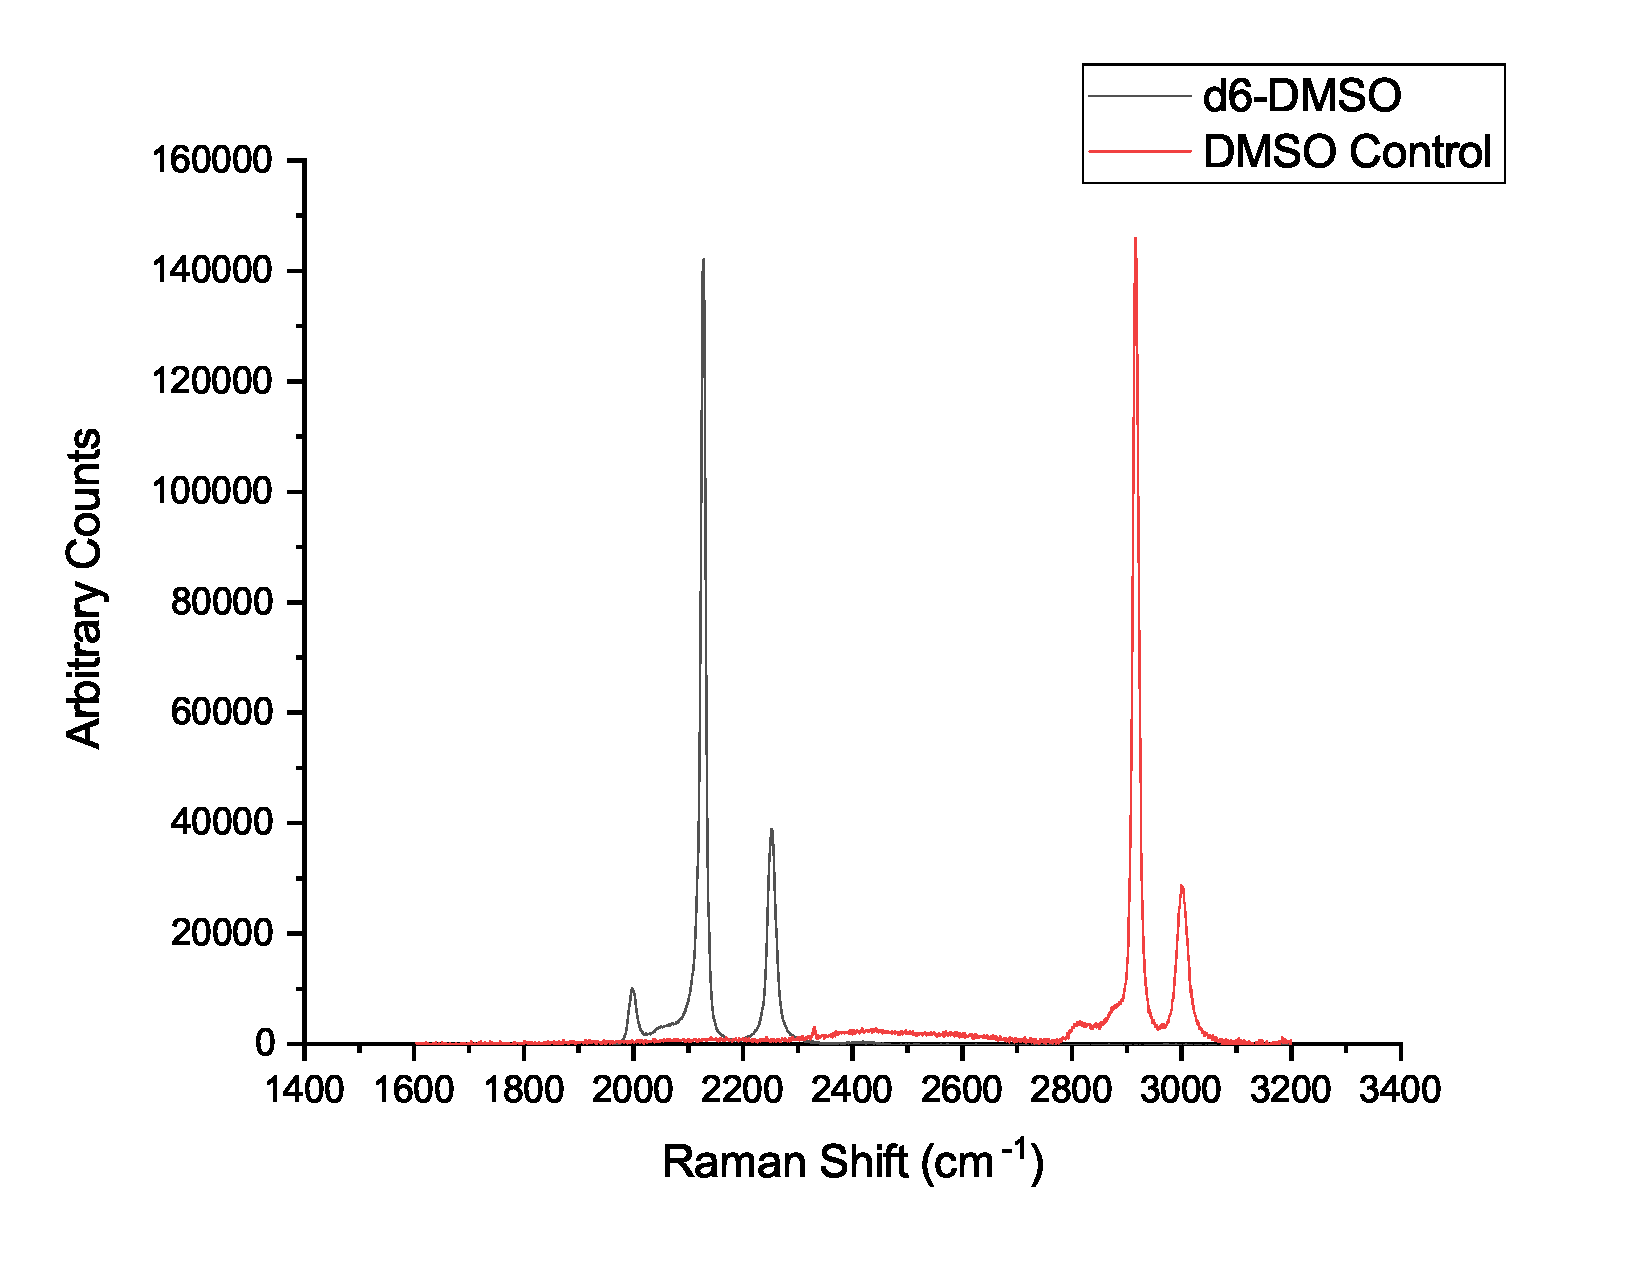
\includegraphics[width=.7\linewidth]{Figures/dmso.eps}
    \caption{Raman Spectra of normal DMSO and deuterated DMSO.}
    \label{fig:spec}
\end{figure}

As Raman scattering spectroscopy probes the various vibrations of molecular bonds it is possible to retrieve a large amount of information from the Raman spectrum. An example of the spectra of DMSO and it's deuterated version are provided in Figure \ref{fig:spec}.~\cite{C6RA25879D} In these spectra, functional group vibrational modes are recognizable in the form of the CH modes centered around 2900$cm^-1$. The comparison of these two spectra show how a slight adjustment in the reduced mass of the oscillator, in this case substituting deuterium for hydrogen, makes a large difference in the position of the Raman peaks.  Detailed analysis of hyperspectral images in SRS, such as that provided with principle component analysis, can utilize this information to produce chemical contrast for images by varying the wavelength of the pump beam over a series of images. In fact, as shown in \cite{Alfonso-Garcia2015}, a range much smaller than that shown in \ref{fig:spec} can provide enough information to sort out differences in compounds such as protein and lipid. Additionally, rapid imaging at one band is available on the order of one frame per second. This creates the ability of SRS to generate images mapping the location of select functional groups in cells and tissues. 

\begin{figure}[ht]
    \centering
    \includegraphics[width=0.5\linewidth]{Figures/dchol.png}
    \caption{SRS imaging at  2120 $cm^-1$ corresponding to CD2 stretches and 2841 $cm^-1$ corresponding to CH2 symmetric stretches. The result of hyperspectral SRS imaging and multivariate analysis is depicted in yellow for D38-cholesterol in the CD region , overlaid on the maximum intensity projection of the CH spectral scan in gray scale, and in red for lipid and green for protein in the CH region.}
    \label{fig:dchol}
\end{figure}

As will be discussed in the section on current work, the addition of small molecule or isotopic tags allows for high chemical contrast not otherwise present in the cell.  An example of this is provided in \ref{fig:dchol} from a previous project in our lab.\cite{Alfonso-Garcia2015}  This image shows how SRS imaging over only a narrow range of wavelengths allows for the colocalization of cholesterol in lipid droplets after esterification. Additionally, as the image shows, with high enough spectral resolution it is possible to separate protein and lipid just based on their signatures in the CH spectral region.








 




 
% Chapter Template

\chapter{A Body of Original Work} % Main chapter title

\label{Chapter3} % Change X to a consecutive number; for referencing this chapter elsewhere, use \ref{ChapterX}

%----------------------------------------------------------------------------------------
%	SECTION 1
%----------------------------------------------------------------------------------------

\section{Previous Work: Deuterium Tags to Study Lipogenesis in A New Cell Type}
This section describes recent work that was completed in collaboration with the research group of Prof. Maxim Plikus.  This work applies SRS microscopy to the study of lipid metabolism using deuterated glucose as a precursor molecule. The cell of interest is the lipochondrocyte, a previously under-described cell found in the ears of small mammals.  These cells are characterized by the presence of a large single droplet that consumes nearly the entirety of the cell. Several experiments were performed in which it was demonstrated that deuterium tagging of small precursor metabolites is a viable strategy for monitoring uptake and metabolism.  It was demonstrated that uptake of glucose from the environment is an active pathway from which lipogenesis occurs in this cell type. Additionally, this study showed the viability of using excised tissue in culture with deuterated compounds.  This expands the ability of the technique to tissues in addition to cultured cells. This work is currently in the manuscript stage and is expected to be submitted for review by the end of the current year.

\begin{figure}[h]
    \centering
    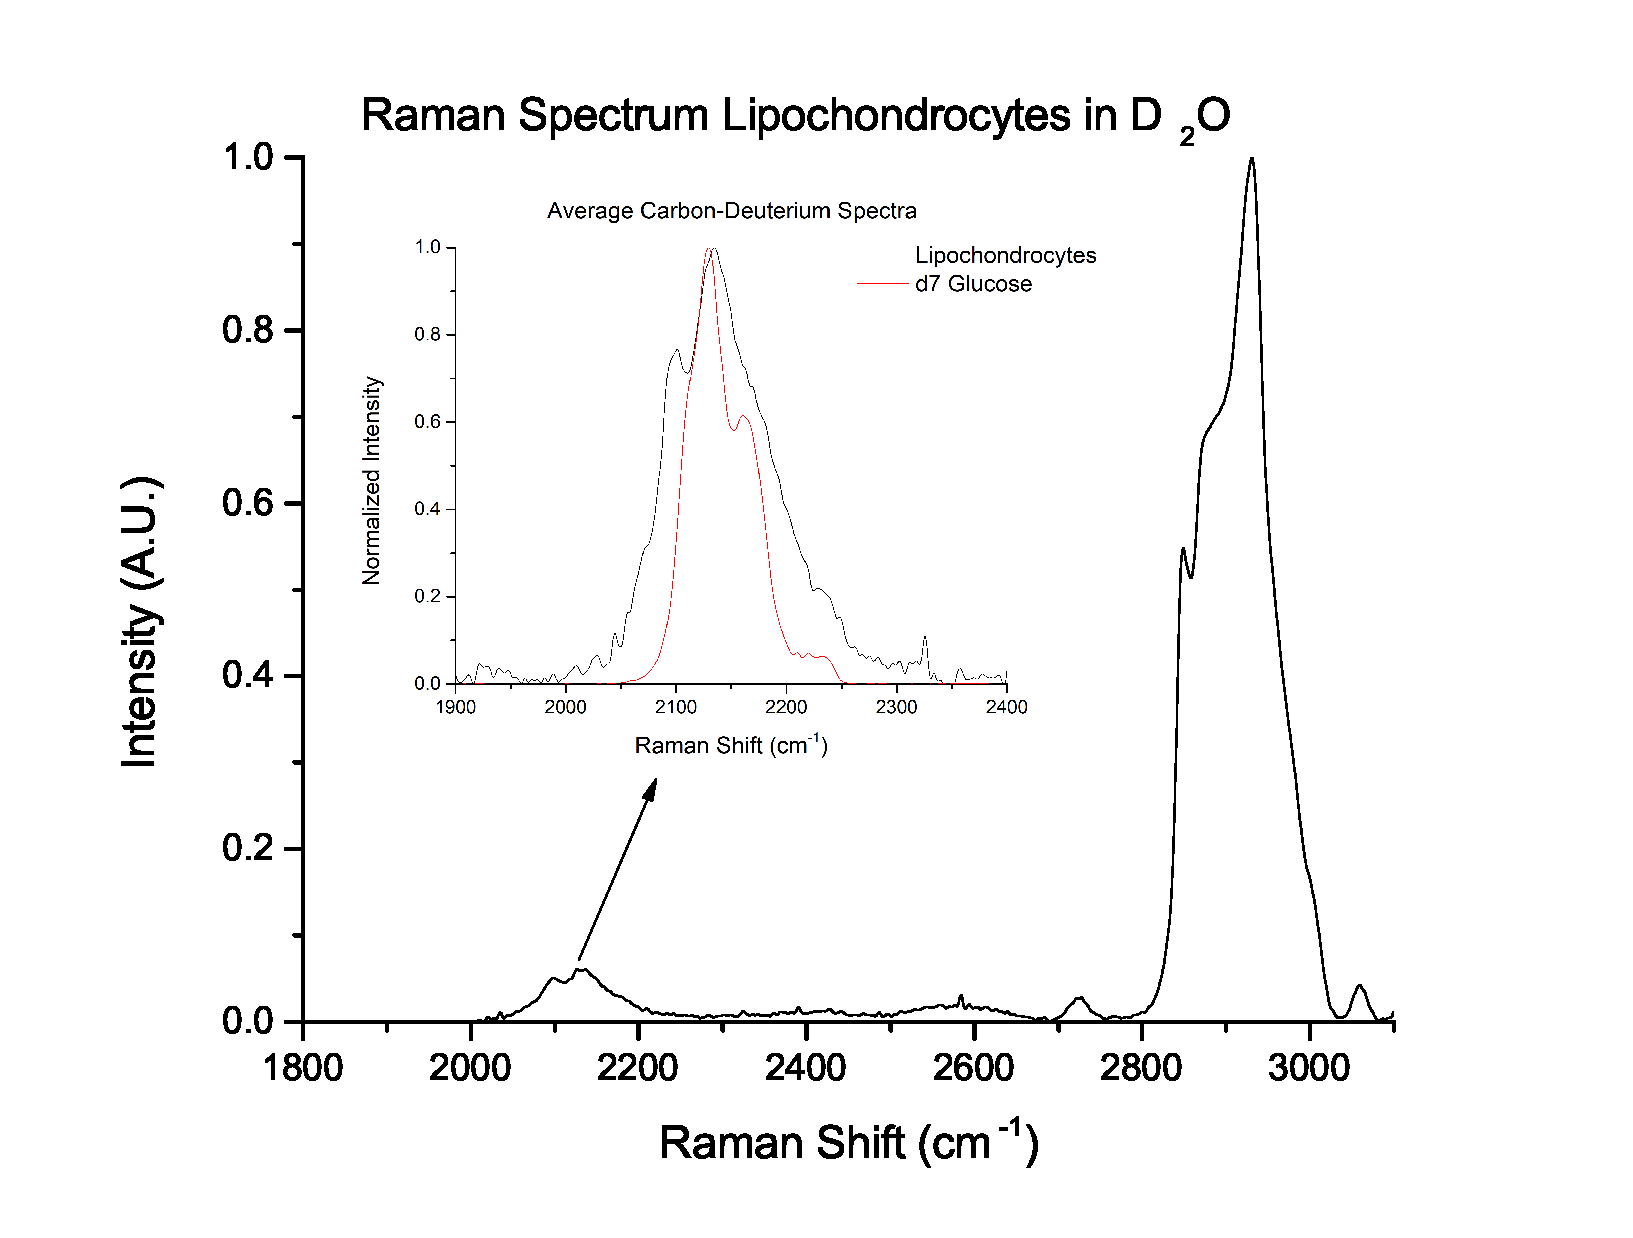
\includegraphics[width=1\linewidth]{Figures/Multigraph.eps}
    \caption{Caption}
    \label{fig:d7multiple}
\end{figure}

Previous work on the use of deuterium tagged molecules has been carried out by members of the Potma group as well as several other groups.~\cite{Hou2503,Alfonso-Garcia2015,Wei:2016aa}  The studies have indicated that deuterium is a useful tool as a contrast agent to mark specific compounds within cells and tissues. My work with the Potma lab was to extend this technique to the study of metabolism, with the lipochondrocyte as the cell model. Specifically, my research question was to examine whether or not the fate of deuterated carbon from a precursor molecule could be tracked in lipochondrocytes with SRS. The first indication that this would be a possibility is borne out in the Raman spectrum of deuterated glucose which is shown in the insert of \ref{fig:d7multiple}. In the first set of experiments excised tissue was cultured in media supplemented with d6-glucose for 48 hours.  The tissue was then fixed with $4\%$ paraformaldehyde and then rinsed.  The tissues were mounted between a standard microscope cover slide and a number 1 coverglass.  Raman spectra were taken from various points of multiple cells on a Renishaw InVia Raman Microscope at the UCI Laser Spectroscopy Facility. In the spectrum taken , we see an intense band centered around $\sim2900cm^{-1}$ from the averaged spectrum taken from the lipochondrocytes. This is attributed to the CH$_2$ stretching modes present in lipids and protein in the cells.  Another peak is present centered around $\sim2140cm^{-1}$  This peak corresponds to the C-D mode present in the cells.  This provides validation that SRS imaging of carbon-deuterium uptake is indeed possible.  The Raman spectrum of the CD modes obtained from the cells shows a marked change from the Raman spectrum of pure d6-glucose. This implies that d6-glucose has been chemically modified. The resulting spectrum shows features characteristic of deuterated lipid, thus suggesting that the majority of precursor molecules are likely converted to lipid-like compounds. 

\begin{figure}[h]
    \centering
    \includegraphics[width=0.5\linewidth]{Figures/2-methyl.jpg}
    \caption{Excised tissue imaged at the CH band.  Image shows primarily lipochondrocyte cells.}  
    \label{fig:Lipo-Methyl}
\end{figure}

After the initial spontaneous Raman study, SRS imaging was performed.  Initially, the system was tuned to the CH band around $\sim2900cm{^-1}$.  These images confirmed the presence of lipids in both control samples incubated with regular glucose and in those tissues cultured in the deuterated glucose media.  Figure \ref{fig:Lipo-Methyl} shows one such image from the deuterated sample set. The phase of the lock in demodulation is set prior to image acquisition to match the SRS signal of long chain fatty acids by first imaging a test sample of oil and adjusting lock-in settings to maximize the signal-to-noise ratio. The field of view of this image shows nearly all cells in this field of view are lipochondrocytes, and the contrast available at this band allows for discrimination of the cells from their surroundings. Figure \ref{fig:4chlipo} shows an image acquired at higher magnification. In this image it is possible to clearly see individual cells, and in some it is possible to see a dark region that is identified nucleus of the cell.  These images were compared with other tissues stained with Bodipy to identify concentrations of neutral lipids, and the same morphology is seen in both sets of samples.

\begin{figure}
    \centering
    \includegraphics[width=0.5\linewidth]{Figures/4-methyl.jpg}
    \caption{Magnified view of lipochondrocytes imaged at the CH band.}
    \label{fig:4chlipo}
\end{figure}

After confirming morphology using the CH region, the SRS was tuned to probe the carbon-deuterium stretch around $\sim2140cm{^-1}$.  For signal optimization, a test sample of deuterated dimethyl sulfoxide was used, and demodulation of the lock in was phase locked to this signal.  Figure \ref{fig:compare} shows the results of one set of images.  Images were successfully acquired in the carbon deuterium band.  Overlay of the images show that the signal of the CD band is co-localized with the signal from the large lipid droplets. Further tests were performed in order to confirm that the signal is indeed from carbon-deuterium oscillators.  The large circular area in the center of the field of view is a collagen filled area.  In these images, it is devoid of cells, however in many instances these contain adipocytes.  Background images were acquired by tuning the OPO off-resonance from any known peak. These images were subtracted from the on-resonance images in order to improve the signal to noise ratio.  

\begin{figure}
    \centering
    \includegraphics[width=\linewidth]{Figures/comparison.png}
    \caption{Lipochondrocytes imaged at both the CH, $\sim2900cm^{-1}$ and CD, $\sim2140cm^{-1}$ regions.  Images show colocalization of the lipid signal and the carbon deuterium signal}
    \label{fig:compare}
\end{figure}

These results lend evidence to the idea that lipid accumulation in lipochondrocytes occurs primarily through de novo lipogenesis as no significant amount of lipds are present in the growth media.  Images acquired at earlier time points in the incubation show decreased CD signal and decreased size of individual lipochondrocyte cells.  In addition to the control and CD groups presented here, our collaborators also performed experiments in which de novo lipogenesis was inhibited through application of C75 which inhibits synthesis of fatty acids. However, if lipid accumulation occurred through the ingestion of environmentally present lipids significant growth and signal would be expected to be present. Figure \ref{fig:pubfig} shows part of a figure intended for publication.  In it the average area of the ears of mice is calculated after application of a control of DMSO and several lipid inhibitors.  This evidence provided by the SRS experiments above lend credibility to the hypothesis that lipid accumulation in this cell type is through lipogenesis.

\begin{figure}
    \centering
    \includegraphics[width=\textwidth]{Figures/paperfig.png}
    \caption{Application of lipogenesis inhibitors to the ears of mice.  Application of C75 inhibits the production of fatty acids leading to deformed ears.}
    \label{fig:pubfig}
\end{figure}

\section{Aim 1: Elucidate diffusion dynamics of common cryoprotectants}
   The use of cryoprotectants to store cell cultures long term is well known, and has applications to fundamental and developmental biology, clinical medicine, stem cell treatments, and work on fertilization.\cite{EGLI2003352,SCHELLANDER1994909,JACOB198614}  Common chemicals used as such include glycerol and dilute concentrations of dimethyl sulfoxide.\cite{Pegg:2002aa}  While it has been established that these chemicals minimize ice crystal formation in the intracellular space, the mechanism by which this is accomplished is debated within the literature.\cite{nucleation1993} Glycerol and DMSO have both been shown to interact with the fusion of liposomes upon thawing, and the choice of cryopreservant can serious effect the viability of cells.~\cite{ANCHORDOGUY1987324, SCHELLANDER1994909} Figure \ref{fig:crystal} shows research on ice crystal formation in preserved cartilage cells images c and d show extensive damage after thawing from the formation of these crystals.~\cite{PEGG2010S36}
   
   Most of the SRS literature presents cases of research in which cells are fixed, or if live, the imaging is done on very specific cases.  In this project, I am proposing to use deuterated DMSO to perform flow based experiments on a variety of cell types.  To consider this project a success, I have identified three goals.  The first is to determine the diffusion coefficient of DMSO through the intracellular space. The results This parameter has been the subject of simulation.\cite{LEEKUMJORN20061751}  The second is to examine localized concentrations of DMSO within cells, and co-localize those concentrations with the distribution of organelles.  The final goal is to examine cells during standard thawing procedures to watch the outward diffusion of DMSO through the plasma membrane.  I expect that these experiments will provide new insights on the biophysical properties of small molecule cryopreservants. 
   
   \begin{figure}[h]
       \centering
       \includegraphics[width=.6\linewidth]{Figures/crystals.jpg}
       \caption{The appearance of control cartilage, sectioned and stained with toluidine blue, is shown in Panels A and B. Panels C and D show cartilage that was cooled to $ -80  \degree C$, freeze-substituted at that temperature, and also stained with toluidine blue. Note the large ice crystal cavities located in chondrons. ($bar = 50$ $\mu m$ in A and C, $bar = 10$ $\mu m$ in B and D) Modified from \cite{PEGG2010S36}.}
       \label{fig:crystal}
   \end{figure}
   
   Coherent Raman techniques have a history in the literature of being used for flow based experiments studying diffusion.  In 2001, CARS microscopy was used to study intracellular water diffusion.~\cite{Potma:2001aa}  Figure \ref{fig:flow} is from the 2001 work and provides an illustration of how the diffusion constant can be obtained through the use of coherent Raman techniques.  More recently in 2017 CARS was used to elucidate the barrier nature of the arterial wall, and was selected for commentary which was authored by myself and E. O. Potma. ~\cite{Lucotte4805, Prince201704101}  In both of these cases, deuterium oxide, heavy water, was used to provide the contrast necessary to follow the flow of water through the cells and tissue.  
   
   \begin{figure}[h]
       \centering
       \includegraphics[width=\textwidth]{Figures/flow.png}
       \caption{Time based imaging of the flush of heavy water in the intracellular and extracelluar space. The time trace in the graph establish the flow of water prior to flush with deuterium oxide and post flush.  This allows for the diffusion time constant to be extracted.}
       \label{fig:flow}
   \end{figure}
   
   Early attempts at conducting this research have proven to be challenging.  As mentioned in the theory section, high-resolution SRS images without spurious background signals require the use of high numerical aperture objectives and condensers.  By definition, these optics have very small working distances.  For the purpose of flow experiments this limits the size of the fluidic systems that can be used. Imaging at steady state after introduction with deuterated DMSO reveals negative contrast in some areas of cultured MCF-7 cells.  This is shown in Figure \ref{fig:MCF7}  The low quality of this image shows that more work in engineering a suitable flow system is needed.
   
   
 \begin{figure}[h]
     \centering
     \includegraphics[width=.5\textwidth]{Figures/3DMSO.jpg}
     \caption{Imaging at the Carbon-Deuterium band reveals inhomogeneous distribution of DMSO through the intracellular space of several MCF-7 cells.}
     \label{fig:MCF7}
 \end{figure}

Current work on this project is focusing on the redesign of our flow cell system.  After several attempts at manufacturing a microfluidic system, a modification of a commercially available system from Bioptechs Corporation is being designed and manufactured. A schematic of the flow system is available in Figure \ref{fig:flowcell}.  The modifications to this system include widening the aperture on the condenser side to accommodate the space requirements of the high-NA condenser.  The system is being made thinner to accommodate the necessarily short working distances of the SRS system optics. Finally, a mounting plate is being designed and machined to accommodate the flow cell into the stage of the SRS microscope.   

\begin{figure}
    \centering
    \includegraphics[width=.5\linewidth]{Figures/flowcell.jpg}
    \caption{Schematic of the Bioptechs flowcell system.}
    \label{fig:flowcell}
\end{figure}

Once the modifications to the flow cell design are accomplished, a process that should be completed by the end of this year, I intend to commence initial experiments with controlled flow.  The inclusion of shaped gaskets in the system allow for controlled nearly laminar flow over the cells.  Perfusion will be accomplished with the use of a syringe pump capable of pushing very low flow rate.  This will allow for repeatable imaging.  From a series of these experiments I expect to be able to collect data on the diffusion of deuterated DMSO across the plasma membrane thus accomplishing the first goal of this project.  

Extensive literature exists on the effects of DMSO on model membranes.\cite{ANCHORDOGUY1992117, GORDELIY19982343} Simple models based on Fink's law are commonplace in literature, and can be used as a starting point before expanding.\cite{LEEKUMJORN20061751} The literature has noted that it is quite common for the diffusion coefficient to be overestimated in small molecules.\cite{Evans:2018aa}  Common values for the diffusivity of DMSO in water range between 0.8 and 1.2 $x 10^-5 \frac{cm^2}{s}$\cite{IECR1992, doi:10.1002/cphc.201500670}  This rate is expected to be hindered based on the results described for intracellular water.

In order to accomplish the second goal of the project, only slight modifications to the SRS system should be necessary.  I intend to use cell cultures with various organelles tagged with fluorescent probes to study the accumulation of deuterated DMSO in and around various organelles. Simultaneous images between the SRS system and the fluorescent detection system will allow for this goal to be met. Interestingly enough in Figure \ref{fig:MCF7} high intensity spots can be seen in several of the MCF-7 cells.  Investigating these high concentration areas will determine what areas of the cell should be investigated in more detail.

Finally, the third goal of this project is to examine the reverse flow of DMSO out of preserved cells. This will be accomplished through the use of the heating element included with the flow cell. By monitoring the the thawing process it should be possible to understand if damage occurs to the cells prior to that point or during.  Additionally, experiments may be performed looking at the usual CH channel for lipids to monitor disruption in lipid droplet distribution during this process. 

It is anticipated that this project will commence in earnest in January 2019.  As stated above, the modifications to the flow system are already underway.  Once experiments begin, this project should take approximately 4 months to complete.  The largest factor with regards to time is maintaining proper cell cultures in order to have repeatable experiments.  Preliminary data should be available by the end of January and the project timeline will be examined and adjusted at that point.

\section{Aim 2: Demonstrate a method for metabolic sorting based on SRS imaging}

This project seeks to demonstrate a method for sorting inhomogenous cultures of cells based on metabolic signatures.  The idea for this project was encouraged through a serendipitous observation during the lipochondrocyte imaging project.  As shown in Figure \ref{fig:twocell} two different cell types are clearly visible.  The set of bright cells in the center of the dark region are immature adipocytes.  Despite the lipochondrocytes large concentration of lipids, the adipocytes are shown to have an even higher uptake of deuterated glucose and conversion to lipid.  This manifests in the much higher signal intensity shown in this image. The higher concentration of deuterated lipid signifies a higher metabolic rate of glucose consumption for the adipocyte cell relative to the lipochondrocyte cell. 

\begin{figure}[h]
    \centering
    \includegraphics[width=0.7\textwidth]{Figures/twocell.jpg}
    \caption{Lipochondrocytes surrounding a small adipocyte.  Both cell types have been cultured in d6-glucose supplemented media.  However, the adiopocyte shows increased signal activity in the deuterium band.}
    \label{fig:twocell}
\end{figure}

In addition to the serendipitous result described above, recent work from the Min group at Columbia University has shown that by culturing cells in heavy water based media a fairly large number of deuterium based peaks show up in the normally silent region of the Raman spectrum.  These peaks can be measured rapidly and the intensity of them can be compared on a per cell basis. These ratios will then be used to devise an algorithm for classifying based on the metabolic rates represented by the Raman peaks.  Included in Figure \ref{fig:ming} are the results from the Min group showing the possibility of using several different deuterium modified functional groups for SRS imaging.~\cite{Shi:2018aa}

\begin{figure}[h]
    \centering
    \includegraphics[width=\linewidth]{Figures/mingraph.png}
    \caption{Caption}
    \label{fig:ming}
\end{figure}

The first goal for this project is to measure the CD peak in a cancer cell line known to experience the Warburg effect, and compare this to a non cancerous line.  All cells will be grown with heavy water supplementation. Additionally, as long as the heavy water is kept at a low percentage of the overall media, the cells are not expected to experience significant isotope effects.  For the first series of experiments, the breast cancer line MDA-MB231 has been chosen.  This line shows increased metabolism as well as easily identifiable lipid droplets.  We will compare the results to cells derived from primary mammary epithelium, which represent healthy cells with a low glycolytic rate.  We expect that the overall amount of carbon-deuterium bonds is significantly different between the two cell types, which thus represents a marker for the metabolic activity of the cultures. The cell culture will be done in collaboration with the group of Prof. Robert Spitale

The second phase of this project will consist of examining mixed cultures of cells.  Cells with an increased metabolism phenotype will be cultured mixed with cells of a less active phenotype.  Using the data collected in the first phase, cells will be examined for the CD peak as well as any others that are found to be relevant.  A classification algorithm will be developed to increase the throughput of the system.  Validation at this step will consist of transfecting the high metabolism phenotype to express a fluorescent marker that can be imaged during the same session as SRS.  This process will be iterative until a high success rate is found.

The final phase of this project will consist of work with several collaborators to develop a microfluidic based sorting system.  In such a system, cells would be flowed through the focus of the microscope system. Based on the spectroscopic data collected previously, the algorithm will decide if the cell is high metabolism or low and the cell will be sorted into an appropriate bin.  Through fluorescent tagging of one of the two cell types this sorting system can also be validated in an iterative process.  

\section{Aim 3: Characterize Third-Order Sum-Frequency Generation as applied to biological systems}

In the past year, our group has published several papers on the development and demonstration of a new multi-modal microscope.\cite{Hanninen:18}  This system is capable of imaging using a new modality, third-order sum-frequency generation (TSFG) in addition to the already demonstrated modalities of SFG and CARS.  The Jablonski diagrams for these three modalities are shown in Figure \ref{fig:my_tsfg}.  In TSFG, molecules are driven at IR-active resonances but are probed through a hyper Raman interaction, effectively up-converting the signal from the IR to the visible range of the spectrum.  This is potentially revolutionary development as it allows IR-based imaging using collection and detection optics that are widely available for use in the visible range. In addition, the two-photon up-converting step confines the probing spot in three dimensions, producing a lateral resolution better than $0.5 \mu m$, many times below the IR-diffraction limit.  As this technique is only recently demonstrated, there remains a large about of work left to further characterize it.  

\begin{figure}
    \centering
    \includegraphics[width=\linewidth]{Figures/tsfg.png}
    \caption{Three different nonlinear optical interactions with vibrational sensitivity. (a) SFG, a second order process sensitive to modes with both Raman and IR activity; (b) CARS, a third order process sensitive to Raman active modes; (c) TSFG, a third order process sensitive to IR-active modes.}
    \label{fig:my_tsfg}
\end{figure}

Like the CRS techniques described above, TSFG depends on the  $\chi^(3)$ nonlinear susceptibility of the molecules under investigation.  Previous work on TSFG has shown that the response of commonly investigated substances like water and lipid have very different responses than would be expected from work done in CARS.  The non-resonant component of the signal is stronger in TSFG but varies from material to material. In order to characterize this, a series of spectral investigations will be carried out on common compounds that are expected to be probed by the microscope. Materials that are expected to be commonly encountered in TSFG experiments are representative solvents (water, ethanol, dimethyl sulfoxide, cyclohexane), biochemical structures (triglyceride, cholesterol, phospholipid, bovine serum albumin, collagen, cellulose, dextrose, DNA), polymer materials (polystyrene, polymethyl-methacrylate, melamine, polyvinyl alcohol), and inorganic materials (borosilicate glass, quartz, titanium oxide). The OPO that supports this system allows for spectral resolution at $\sim10cm{^1}$, and the spectra will be collected over a range of 2080 to 4000 $cm^{-1}$.  These spectra will be correlated with spectra collected from UV/Vis and FTIR.  The UV spectra correlation will provide information on the effect of proximity to electronic resonances on the TSFG response.  The FTIR spectra will serve to inform the resonant response of the material much as the spontaneous Raman spectra does in SRS or CARS investigations.

The second phase of investigations with this system will be its application to biological systems.  In particular, this system will be applied to work from our longstanding collaboration with Prof. James Jester (Ophthalmology, UCI), which focuses on the distribution and composition of lipids in the meibomian gland.  Meibum has previously been investigated with SRS, and those studies revealed new information about the distribution of protein and lipid in meibum with applications towards understanding dry eye disease.  Hyperspecral imaging through TSFG will provide protein/lipid distribution maps.  These will be compared and correlated with the maps originally derived from SRS investigations.  This will reveal additional information about the composition of the lipids in the meibomian gland and their role in the tear film layer of the eye.

The timeline for this project will commence during the second half of 2019.  At that point, collection of data on the various compounds will commence.  This part of the project along with optimization of the TSFG system itself will last for the remainder of the year.  Collection of UV/Vis data and FTIR will be conducted at the UCI Laser Spectroscopy Facility and will be conducted by a pair of highly trained undergraduate students currently working in the lab.  This will free graduate researcher time to focus on the TSFG system itself. Work on the meibum system will commence in early 2020 and last for an expected six months.

% Chapter Template

\chapter{Summary of the Research Plan} % Main chapter title

\label{Chapter4} % Change X to a consecutive number; for referencing this chapter elsewhere, use \ref{ChapterX}

%----------------------------------------------------------------------------------------
%	SECTION 1
%----------------------------------------------------------------------------------------

In this proposal I have outlined a plan of original research to fulfill the dissertation requirements of the Ph.D. program in Biomedical Engineering.  Through the development and application of vibrational imaging, this work will elucidate several problems in biological physics.  The first two projects are roughly divided towards a pure science aim to investigate diffusion of cryoprotectants, and an applied science project in developing a sorting system based on signals derived from cellular metabolism.  The third project expressly extends the field of vibrational imaging by continuing on work that I've already started on the implementation of a new modality in the form of TSFG.  Characterizing that system will lead to immediate contributions to the field of biological imaging.

Based on the projects proposed here the format of my dissertation seems evident.  The first chapter shall examine the state of vibrational imaging with a focus on stimulated Raman scattering theory and application.  This chapter will be based in large part on the review article already published.  The second chapter will focus on the application of SRS and deuterium labeling to the characterization the new cell type known as lipochondrocytes.  As this work is soon to be sent for review, it will  not require much more effort to extend it to the level of a dissertation chapter.  Each of the three projects proposed here will be developed through the proposed investigations into a chapter each.  Additionally, as each of these projects is already begun in some preliminary form it is expected that they will each take a devoted amount of time of around six months.  This falls well into the schedule of my remaining program.  Completion of these projects within that time line would have me completing my dissertation around the end of the Summer 2020 term. This would be well withing the normal time to degree for students in the biomedical engineering program 
%\include{Chapters/Chapter5} 

%----------------------------------------------------------------------------------------
%	THESIS CONTENT - APPENDICES
%----------------------------------------------------------------------------------------

\appendix % Cue to tell LaTeX that the following "chapters" are Appendices

% Include the appendices of the thesis as separate files from the Appendices folder
% Uncomment the lines as you write the Appendices

%\include{Appendices/AppendixA}
%\include{Appendices/AppendixB}
%\include{Appendices/AppendixC}

%----------------------------------------------------------------------------------------
%	BIBLIOGRAPHY
%----------------------------------------------------------------------------------------

\printbibliography[heading=bibintoc]

%----------------------------------------------------------------------------------------

\end{document}  
